\documentclass[a4paper,11pt]{article}

\usepackage{url}
\usepackage{graphicx}

\title{PeerSim HOWTO: build a new protocol for the peersim simulation
framework}
\author{Gian Paolo Jesi (jesi@cs.unibo.it)}
\date{November 10, 2005}

\begin{document}

\maketitle



\section{Introduction}

\textbf{NOTE: This tutorial revision covers peersim release 1.0
  topics.}\\


\textbf{NOTE: if the reader is not a peersim newbie, she may be
  interested in which major changes have been introduced; a small, but
  fast reference is provided in Appendix
  \ref{sec:Appendix-C-changes}. For deeper details, check the peersim
  CHANGELOG file.}\\


This tutorial is aimed to give you a step by step guide to build from
scratch a new peersim application
(\url{http://sourceforge.net/projects/peersim}): 
a framework to experiment with large scale P2P overlay networks. In
this tutorial it supposed that you and/or your workstation have: 

\begin{itemize}
\item knowledge of O.O. programming and Java language;
\item a working Java compiler ( $\geq$ JDK 1.5.x);
\item a 1.0 peersim release package or a working peersim source tree
  (you can download it from sourceforg CVS);
\item the Java Expression Parser version $\geq$ 2.3.0 (download it from: \url{http://www.singularsys.com/jep/});
\item (suggested) gnuplot software. 
\end{itemize}

The aim of this tutorial is to be
as practical as possible; the goal is to give the reader the basics
of peersim usage and the basics about howto write a simple component.
This tutorial IS NOT exhaustive at all!\\

Because of the spiritus of this tutorial,
after a brief introduction to basic concepts, we will try to learn peersim
and its basic components
using a by example methodology.


\section{Introduction to Peersim}


\subsection{Why peersim}

One of the P2P system properties is that they can be extremely large
scale (millions of nodes); another issue to deal with, is the high
dynamism of such systems: nodes in the network join and leave continuously.
Setting up a protocol experiments in a such simulated environment it
is not an easy task at all.

Peersim has been developed to cope with these P2P properties and thus
to reach extreme scalability and to support dynamism. In addition,
the simulator structure is based on components and makes easy to fast
prototype a simulation joining together different pluggable building
blocks. The term \char`\"{}components\char`\"{} used here has no relation
with high level component architectures (e.g.: CORBA, DOM+).

The peersim performances can be reached only assuming some relaxing
assumptions about the simulation details. For example, the overhead
introduced by the low level communication protocol stack (e.g.: TCP
or UDP) in not taken into account because of the huge additional memory
and CPU time requirements needed to accomplish this task. Another simplifying
assumption is the absence of concurrency: in peersim the simulation
is sequential and based on the concept of cycle in which every node
can select a neighbor (the neighborhood relation could be defined
by a fixed topology or defined by an overlay management protocol such
as \emph{Newscast}) and perform a protocol defined function.


\subsection{Peersim simulation life-cycle}

The peersim structure is aimed to promote modular programming of building
blocks. Every such block is easily replaceable by another component
having a similar function, that means, in brief, having the same interface.
In the peersim framework, a simulation is carried by the \emph{Simulator}
class. The general idea of the simulation model is: 

\begin{enumerate}
\item choose a network size (number of nodes); 
\item choose 1 or more protocol to experiment with and initialize
the protocol(s); this step will build a topology on top of raw nodes
inserted at the previous point;
\item choose 1 or more \emph{Control}\footnote{The \emph{Control} is
  the unified interface that substitutes the old \emph{Observer} and
  \emph{Dynamics} interfaces.}
 object to monitor the properties
  you are interested in and to modify or perturb some parameter during
  the simulation execution (e.g.: the size of th
network, update particular values inside protocols, ...); 
\item ... run your simulation invoking the \emph{Simulator} class
\end{enumerate}

This is a very general model to give the reader an idea to start with,
but the simulation scenario can be extremely more complex. 

All the object created during the simulation are instances of classes
that implements one or more well defined framework interfaces. The
main interfaces I suggest you to become familiar with are in the
Table~\ref{t:psim_classes}.


\label{table1}
\begin{table}
\begin{center}\begin{tabular}{|c|p{2.5in}|}
\hline 
\emph{Node}&
All the elements of a P2P network are called nodes, the interface
manages the local view of neighbor, the reference to the protocol,
its index identifier inside the topology global array (invisible to
protocols)\\
\hline 
\emph{CDProtocol}&
A protocol simply defines an operation to be performed at each cycle
(only method nextCycle() is defined)\\
\hline 
\emph{Linkable}&
A class implementing this interface has access to the underling network:
can access to its local view of neighbor\\
\hline 
\emph{Control}&
Is a very general interface to run any kind of code using its
\emph{execute()} method. In general, it is the base interface to observe or
modify the simulation\\
\hline
\emph{Vector}&
Is a package of classes aimed to modify and analyze numeric vectors
defined by the vector of protocol instances in the overlay. All the
protocol instances contained by nodes in the network define a protocol
vector. These classes handle protocol vectors as a whole: for example,
by observing one of its fields and reporting aggregation statistics
over them. \\
\hline
\end{tabular}\end{center}

\caption{\label{t:psim_classes}Suggested peersim subset of classes or
  interfaces to know about.} 
\end{table}


The life-cycle of a peersim simulation is hard coded inside the
\emph{peersim.Simulator} class. It first reads a particular
configuration file (see section 
\ref{configfile}) containing all the simulation parameters 
concerning all the
objects involved in the experiment. If no error occurs, the simulator
loads and executes \emph{Control} type objects. A special
\emph{Control} object (\emph{peersim.cdsim.FullNextCycle}) is
dedicated to actually run the protocols.
From a developer point of view, it is important to note that the
protocols creation process is based on \textbf{cloning}: only one instance
of each protocol is actually forged (with the \textbf{new} statement)
and then it is cloned to populate all the network. Thus the 
\emph{clone()} method has to be designed with care to avoid 
unpredictable results.

Each object in peersim (controls and protocols) is wrapped into
\emph{Scheduler} objects which adds fine grained scheduling facilities to each
simulation component. This approach leads to total freedom in the
cycle execution. For example, it is possible to run a subset of
protocols at the beginning, then some controls in between and finally
the other protocols (o even a subset). Such kind of scenario is depicted in
Figure~\ref{obsfigure}. 

The initialization phase is carried out by special \emph{Control}
objects that run only at the beginning. To obtain this effect, this
initializer is internally wrapped by the simulator in a \emph{Scheduler} 
class object that ensures a single shot. In the configuration file,
the initialization components are easily recognizable by the
\texttt{init} prefix. Please note that in the following pages we will
talk about \emph{Initializer} objects just to remark their function and
to distinguish them from ordinary \emph{Control} objects, however there
is no \emph{Initializer} class in peersim
\footnote{Class
  \emph{Initializer} was available in early peersim releases, but
  since version 0.3 has been completely removed.}.

%Before executing the protocol code, the simulator runs the \emph{Control}
%object(s), but the developer can choose and define
%the execution order of these components and the cycle interval to
%work in. For example, as depicted in Figure~\ref{obsfigure}, we can
%choose to run one or more \emph{Control} object before and/or one
%5or more \emph{Control} objects after the \emph{Dynamics} object(s).
%Nevertheless, also after the last cycle we can choose to run an
%  \emph{Observer}
%to retreive a final snapshot.


\begin{figure}
\begin{center}
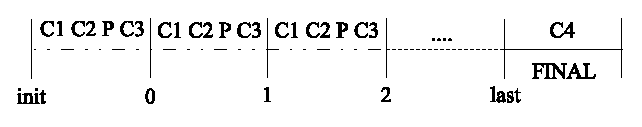
\includegraphics[scale=1.1]{controls-protocols.eps}
\end{center}
\caption{Controls and protocols scheduling. The ``C'' letters indicate
  control component, while letter ``P'' indicates a generic protocol
  execution. The numbers in lower part of the picture indicates the
  peersim cycles. After the last cycle, it is possible to run a final
  control to retrieve a final snapshot.\label{obsfigure}}
\end{figure}


When a \emph{Control} has to collect data, they are formatted and sent to
standard output and can be easily redirected to a file to be collected
for further work. 
%When developing such a \emph{Control} class, a good
%rule is to print out data using the \emph{peersim.core.Log} static class.


\subsection{The config file}
\label{configfile}

The config file is a plain ASCII text file, basically composed of
key-value pairs; the lines starting with \char`\"{}\#\char`\"{} character
are ignored (comments). The pairs are collected by a standard Java
\emph{java.util.Properties} object when the simulator starts using
for example the following command:

\begin{verbatim}
java -cp <class-path> peersim.Simulator config-file.txt \end{verbatim}


Clearly the classpath is mandatory only if you have not set it yet
in a global shell variable.

\subsection{Configuration example 1}

First of all, what we are going to do in this first experiment? 

We are going to impose a fixed P2P random topology composed by 50000
node network; the chosen protocol is \emph{Aggregation} (what is
aggregation? see appendix \ref{sec:Appendix-A-aggregation}) using
an average function. The values to be aggregated (averaged) at each
node are initialized using a linear distribution on the interval {[}0,
100{]}. Finally a \emph{Control} monitors the averaging values.
Looks easy!

\footnotesize
\begin{verbatim}
1 # PEERSIM EXAMPLE 1
2
3 random.seed 1234567890
4 simulation.cycles 30
5
6 control.shf Shuffle
7
8 network.size 50000
9  
10 protocol.lnk IdleProtocol
11
12 protocol.avg example.aggregation.AverageFunction
13 protocol.avg.linkable lnk
14 
15 init.rnd WireKOut
16 init.rnd.protocol lnk
17 init.rnd.k 20
18 
19 init.peak example.aggregation.PeakDistributionInitializer
20 init.peak.value 10000
21 init.peak.protocol avg
22
23 init.lin LinearDistribution
24 init.lin.protocol avg
25 init.lin.max 100
26 init.lin.min 1
27
28 # you can change this to select the peak initializer instead
29 include.init rnd lin
30
31 control.avgo example.aggregation.AverageObserver
32 control.avgo.protocol avg
\end{verbatim}
\normalsize


Lets comment the code line by line. 

The first things to note are the
key names: some of them are referred to global properties, while some
others refer to single component instancies. For example,
\texttt{simulation.cycles} is global, but \texttt{protocol.lnk.xxx}
defines parameter \textbf{xxx} of protocol \textbf{lnk}.

From the previous example, follows that each component instance has a
human readable (e.g., a string) identifier, such as \texttt{lnk}. This
identifier is resolved as an numering index identifier by the peersim
engine, but the user does not have to deal with it. 

A component such as a protocol or a control (or even an initializer
which is a special control case), is declared by  the
following syntax scheme:

\footnotesize
\begin{verbatim} <protocol | init| control> . string_id   [full_path_]classname
\end{verbatim} \normalsize

note that the full class path is optional, in fact peersim can search
in its classpath in order to find the class. If multiple classes share
the same name (in distinct packages), the full path is needed.
  
The component parameters (if any) follows this scheme:

\footnotesize
\begin{verbatim} <protocol | init| control> . string_id [. parameter_name ]
\end{verbatim} \normalsize


The final $<$parameter\_name$>$ is contained between {[}{]} to express
that it is optional. 

For example, at \textbf{line 10}, the first protocol chosen comes to life;
the \textbf{key part} contains its type (or interface type) followed
by the index and \textbf{the
value} part contains the desired component class full package path
(you have to check the javadoc files or the source tree to discover
the correct package path). In the case of a component parameter
declaration (see \textbf{line 13},the \textbf{key part} contains the parameter name and the \textbf{value
part} is simply the value desired (usually an integer or a float).

From \textbf{line 3 to line 8}
some global simulation properties are imposed; these are the total
number of simulation cycles and the overlay network size. The
\emph{Shuffle} control (\textbf{line 6}) is something like a
\emph{system control} needed to shuffle the order in which the nodes
are visited in each 
cycle. 

From \textbf{line 10 to line 13}, two protocols are put in the arena.
The first one, \emph{peersim.core.IdleProtocol} does nothing. It is useful
because of its ability to access to the topology, in fact it provides
neighbour links to each node. This feature is present because \emph{IdleProtocol}
is an implementation of the \emph{Linkable} interface. 

The second protocol (\texttt{protocol.avg aggregation.AverageFunction})
is the averaging flavor of aggregation. Its parameter (\texttt{linkable})
is extremely important: it expresses the need to access the topology
using not this protocol itself (aggregation), but with the
linkable-implementing underlying protocol. This is due to the structure
of aggregation: it does not implement the \emph{Linkable} interface,
so it can not ``see'' the neighbor list by itself and it must use some other
protocol in order to do that. The value of parameter linkable is the identifier
of a \emph{Linkable} interface implementing protocol (\emph{IdleProtocol}
in the example). Clearly to know if a protocol can get access to the
topology directly or not, you have to check the documentation (or source
code).

From \textbf{line 15 to line 26}, it is time to initialize all the
components previously declared. The initialization components
are three, but only two of them are actually used at the same
time. The first initializer, \texttt{peersim.init. WireKOut},
imposes a node wiring (e.g., a topology). The nodes using the declared
protocol are linked
randomly to each-other to form a random graph having the specified
degree (\texttt{k}) parameter. 

The second and third initializer task is to initialize the aggregation
function value-field to be averaged. Respectively, The initialization
values follows a peak and linear
distribution fashion. Both initializers need a protocol identifier to
refer to (\texttt{protocol} parameter) and initialization values
ranges according to their functions (e.g., \texttt{max}, \texttt{min}
parameters 
for the \emph{PeakDistributionInitializer} and \texttt{value}
parameter for \emph{LinearDistribution}). 

The chance to use the peak or linear distribution is given by the
\texttt{include. init} directive (\textbf{line 29}) that selects which
initializers are 
allowed to run following the order in which they have been
inserted. The same directive works also with protocols and controls.

Finally at \textbf{line 31, 32} the last component is declared:
\texttt{aggregation. AverageObserver}. Its only parameter used is \texttt{protocol} and clearly refers to the
\emph{aggregation.AverageFunction} protocol type, so the parameter
value is the \texttt{avg} string-id (means: \emph{aggregation.AverageFunction}). 

Now you can try the example writing on a console the following line:

\begin{verbatim}
java -cp <class-path> peersim.Simulator example1.txt \end{verbatim}

The class-path is mandatory only if the current system has not peersim
classes in the shell CLASSPATH environment variable. To get the exact
output that will follow, the reader should uncomment the parameter
at \textbf{line 3}:

\begin{verbatim} random.seed 1234567890 \end{verbatim}

on top of the configuration file. This parameter is very useful to
replicate exactly the experiment results based on (pseudo) random
behavior. The experiment output is (some initialization strings may
be different):

NOTE: cut and paste the experiment: 

\tiny
\begin{verbatim}
Simulator: loading configuration
ConfigProperties: File example/config-example1.txt loaded.
Simulator: starting experiment 0 invoking peersim.cdsim.CDSimulator
Random seed: 1234567890
CDSimulator: resetting
Network: no node defined, using GeneralNode
CDSimulator: running initializers
- Running initializer init.rnd: class peersim.dynamics.WireKOut
- Running initializer init.lin: class peersim.vector.LinearDistribution
CDSimulator: loaded controls [control.avgo, control.shf]
CDSimulator: starting simulation


control.avgo: 0 1.0 100.0 50000 50.49999999999998 816.7990066335468 1 1
CDSimulator: cycle 0 done
control.avgo: 1 1.2970059401188023 99.38519770395408 50000 50.50000000000005 249.40673287686545 1 1
control.avgo: 2 9.573571471429428 84.38874902498048 50000 50.500000000000085 77.89385877895182 1 1
control.avgo: 3 23.860361582231647 71.93627224106982 50000 50.49999999999967 24.131366707228402 1 1
control.avgo: 4 34.920915967147465 68.92828482118958 50000 50.49999999999994 7.702082905414273 1 1
control.avgo: 5 42.37228198409946 59.94511004870823 50000 50.49999999999987 2.431356211088775 1 1
control.avgo: 6 45.19621912151794 54.855516163070746 50000 50.499999999999844 0.7741451706754877 1 1
control.avgo: 7 47.68716274528092 53.11433934745646 50000 50.49999999999949 0.24515365729069857 1 1
control.avgo: 8 48.97706271318158 52.38916238021276 50000 50.50000000000026 0.07746523384731269 1 1
control.avgo: 9 49.59674440194668 51.46963472637451 50000 50.49999999999937 0.024689348817011823 1 1
control.avgo: 10 49.946490417215266 51.13343750384934 50000 50.50000000000048 0.007807022577928414 2 1
control.avgo: 11 50.18143472395333 50.858337267869565 50000 50.49999999999982 0.002493501256296898 2 1
control.avgo: 12 50.30454978101492 50.67203454827276 50000 50.500000000000206 7.90551008686205E-4 1 1
control.avgo: 13 50.3981394834783 50.60093898689035 50000 50.49999999999967 2.518940347803474E-4 1 1
control.avgo: 14 50.449347314832124 50.54962989951735 50000 50.5000000000003 8.071623184942779E-5 1 1
control.avgo: 15 50.47368195506415 50.52608817343459 50000 50.49999999999999 2.566284350168338E-5 1 1
control.avgo: 16 50.48510475374435 50.518871021756894 50000 50.50000000000012 8.191527862075119E-6 1 1
control.avgo: 17 50.49082426764112 50.51000681641142 50000 50.49999999999945 2.570199757692886E-6 1 1
control.avgo: 18 50.494810505765045 50.50556221303088 50000 50.5000000000003 8.197012224814065E-7 1 1
control.avgo: 19 50.496876367842034 50.50296444951085 50000 50.499999999999524 2.640584231868471E-7 1 1
control.avgo: 20 50.498457906558905 50.50182062146254 50000 50.500000000000334 8.565428611988968E-8 1 1
control.avgo: 21 50.49905541635283 50.50096466374638 50000 50.49999999999974 2.721171621666857E-8 1 1
control.avgo: 22 50.49946061473347 50.500553628252945 50000 50.49999999999975 8.590349265230611E-9 1 1
control.avgo: 23 50.49972602272376 50.500315571370415 50000 50.5000000000004 2.6248542064007986E-9 2 1
control.avgo: 24 50.4998450606816 50.50018053311878 50000 50.50000000000005 8.845012874999227E-10 1 1
control.avgo: 25 50.499894793874255 50.500096923965216 50000 50.50000000000079 1.864501428663076E-10 1 2
control.avgo: 26 50.4999267984512 50.500056126785694 50000 50.5000000000003 8.594896829690765E-11 1 1
control.avgo: 27 50.49996613170552 50.50003198608762 50000 50.50000000000017 1.9554527178661528E-11 1 1
control.avgo: 28 50.49997903068333 50.500019172164286 50000 50.499999999999766 3.274246411310768E-11 1 1
control.avgo: 29 50.49998958653935 50.5000099409645 50000 50.50000000000045 0.0 1 1
\end{verbatim}
\normalsize

The observer component produces many numbers, but looking at the 3th and
4th data columns (respectively the maximum of averages and the minimum
of averages) it is easy to see how the variance decreases very quickly.
At cycle 12, quite all the nodes has
a very good approximation of the real average (50). Try to experiment
with different numbers and then to change the init distribution (e.g.:
using \texttt{aggregation.Peak DistributionInitializer}) and / or the
protocol stack (put \emph{Newscast} or \emph{SCAMP} instead of 
\emph{IdleProtocol}).


\subsection{Configuration example 2}

This second example is an improved version of the first one. What is
new? Now the aggregation protocol runs on top of Newscast and a new
values distribution is provided (simply uncomment it and comment out
the first two lines of the previous distribution). Moreover, there is
a \emph{Control} object that changes the network size, shrinking it by
cutting out 500 nodes each time).

\footnotesize
\begin{verbatim}
1 # PEERSIM EXAMPLE 2
2
3 random.seed 1234567890
4
5 simulation.cycles 30
6
7 control.shf Shuffle
8
9 network.size 50000
10 
11 protocol.lnk example.newscast.SimpleNewscast
12 protocol.lnk.cache 20
13
14 protocol.avg example.aggregation.AverageFunction
15 protocol.avg.linkable lnk
16
17 init.rnd WireKOut
18 init.rnd.protocol lnk
19 init.rnd.k 20
20
21 init.pd example.aggregation.PeakDistributionInitializer
22 init.pd.value 10000
23 init.pd.protocol avg
24
25 init.ld LinearDistribution
26 init.ld.protocol 1
27 init.ld.max 100
28 init.ld.min 1
29
30 # you can change this to include the linear initializer instead
31 include.init 0 1 
32
33 control.ao example.aggregation.AverageObserver
34 control.ao.protocol avg
35
36 control.dnet DynamicNetwork
37 control.dnet.add -500
38 #control.dnet.minsize 4000
39 control.dnet.from 5
40 control.net.until 10
\end{verbatim}
\normalsize

The global parameters are the same as in the previous example; only
new additions are discussed below. At \textbf{line 11-12} there is the
\emph{Newscast} (what is newscast? See Appendix \ref{sec:Appendix-B-newscast}) 
component declaration with its 
only parameter cache (please note: cache size should be at least as
large as network \texttt{k} degree size). 
The initializers section (at \textbf{lines 17-28}) is the same as in
the previous example. However, here the peak distribution is
selected. To change it and switching to the linear distribution,
change the \texttt{include init} directive at \textbf{line 31}.

The
peak distribution initializes all nodes except one with 0 value and
the node left takes the value declared in the \texttt{value} parameter.

From \textbf{line 27 to 32} is present the last new component: 
\texttt{control.dnet
peersim.dynamics.DynamicNetwork}. As stated previously, a \emph{Control}
implementing object can be used to to change some other object
properties; the change can be performed at each simulation cycle (default
behavior) or using a more sophisticated approach. The object chosen
in the example deletes 500 nodes from the net at each time (well,
it is not completely correct to talk about deletion in peersim vision,
since the \emph{Linkable} interface does not support the delete
operation; so it is better to think about \char`\"{}unlinking\char`\"{} 
nodes from the overlay). The parameters \texttt{add}, \texttt{minsize},
\texttt{from} and \texttt{until} have respectively the following meaning:

\begin{itemize}
\item adds the specified number of nodes (if negative, subracts);
\item the minimum size is referred to the overlay: it can not be less than
what is stated here;
\item the cycle number from which the component can start running;
\item the cycle number until which the component object can run.
\end{itemize}

Other parameters are available; please check the source or the JavaDoc.

It is interesting to note that not all the parameters associated to
a \emph{Control} component can be found in its source code (or
documentation); this is due to the Simulator class 
behavior. When it creates the \emph{Control} instances, it
wraps them in a \emph{Scheduler} class object: this is the class where
some parameters (such as \texttt{step}, \texttt{from}, \texttt{until})
are actually defined.

\subsection{Advanced configuration features}

Thanks to the presence of the Java Expression Parser (since release
0.2), the configuration
file can handle many types of \textbf{expressions}, such as boolean 
expressions, common mathematical functions and well known predefined
constants (e.g.: $\pi$ and $e$); for an exhaustive feature list check
the Java Expression Parser web page
(\url{http://www.singularsys.com/jep/index.html}).

Expressions can be used anywhere instead of numeric values, as follows:

\begin{verbatim}
MAG 2
SIZE 2^MAG
\end{verbatim}

the variable SIZE will be auto-magically evaluated in number 4.

Multiple expressions can be written in a tree-like fashion and they will
be evaluated recursively (the CPU conscious users have to know that 
no optimizations are performed and the same expression may be evaluated
many times) as in the following code sample:

\begin{verbatim}
A B+C
B D+E
C E+F
D 1
E F
F 2
\end{verbatim}

The evaluation will produce: A=7, B=3, C=4, D=1, E=2 and F=2.

Recursive definitions are not allowed and a simple trick is used to 
avoid them: if the recursion depth is grater than a configurable 
threshold parameter (set at 100 by default) an error message is
printed and the simulator stops.

For any kind of simulator object (e.g., protocol, control and init),
it is possible to specify an ordering scheme. The default one is given
by the component ids
alphabetically order.
%In fact, the object prefixes are
%not limited to numerical indexes, but they can be expressed by any 
%string, as follows:

\begin{verbatim}
control.conn ConnectivityObserver
control.myClass Class1
control.1 Class2
\end{verbatim}

The lexicographical order can be explicitly overridden 
giving an item name list separated  by any non-word character
(non alphanumeric or underscore) in the following directive:

\begin{verbatim}
order.observer myClass conn 1
\end{verbatim}

If not all names appear in the list,
then the vacant objects will follow the default alphabetical order.
For example:

\begin{verbatim}
order.observer myClass
\end{verbatim}

will produce the following order:

\begin{center}
$\langle$ \texttt{observer.myClass} ; \texttt{observer.1} ;
\texttt{observer.conn} $\rangle$
 
\end{center}

Another available feature is to tell the simulator which items are
allowed to run using the following directive:

\begin{verbatim}
include.control conn myClass
\end{verbatim}

This will return \texttt{control.conn} and \texttt{control.myClass}.
If the list is empty, then an empty ordering array will be
generated; means that, in this case, no controls will run. 

%\subsubsection{A concrete example}

%To have a practical idea about how to use these new features, the following
%example is presented; it is a modified example2 version.

%\footnotesize
%\begin{verbatim}

%1 #random.seed 1234567890
%2 simulation.cycles 30
%3 control.0 peersim.cdsim.Shuffle
%4
%5 # Imposes the correct protocol running order:
%6 order.protocol ncast avgagr
%7 include.control avgobs
%8 
%9 overlay.size 50000
%10 overlay.maxsize 200000
%11 
%12 protocol.ncast example.newscast.SimpleNewscast
%13 protocol.ncast.cache 20
%14
%15 protocol.avgagr example.aggregation.AverageFunction
%16 protocol.avgagr.linkable ncast
%17
%18 init.wrr peersim.vector.WireKOut
%18 init.wrr.protocol ncast
%20 init.wrr.k 20
%21
%22 # UNCOMMENT THE FOLLOWING LINES TO GET A LINEAR DISTRIBUTION
%23 init.ldistrib peersim.vector.LinearDistribution
%24 init.ldistrib.protocol avgagr
%25 init.ldistrib.max 100
%26 init.ldistrib.min 1
%27
%28 control.avgobs example.aggregation.AverageObserver
%29 control.avgobs.protocol avgagr
%30
%31 control.dnetwork peersim.dynamics.DynamicNetwork
%32 control.dnetwork.add -500
%33 control.dnetwork.minsize 4000
%34 control.dnetwork.from 5
%35 control.dnetwork.until 10
%\end{verbatim}
%\normalsize

%In this configuration file, the component indexes are no more used,
%but a string identifier is used instead. 
%Because of the chosen protocol symbol names (\texttt{ncast} and 
%\texttt{avgagr}),
%it is necessary to impose a different running order scheme to let
%newscast run first using (at \textbf{line 6}):
%
%\begin{verbatim}
%order.protocol ncast avgagr
%\end{verbatim}

%In addition, a similar approach is used with the controls for
%observing the simulation (at \textbf{line 7}):

%\begin{verbatim}
%include.control dnetwork
%\end{verbatim}

%This allows only the \texttt{dnetwork} control to run. This approach
%avoids the usage of error prone comments in the file to switch
%components on or off.  

%\section{Writing a new protocol}
%

%This section covers the description of how to write a new protocol. 


\subsection{Which kind of protocol?}

The protocol we are going to develop is a simple load balancing algorithm.
It works as follows. The state of a node is composed of two values:
the local load and the quota. The second one is the amount of ``load''
the node is allowed to transfer at each cycle. The quota is necessary
in order to make real load balancing, otherwise it would be simply
averaging. Every node contacts the most \textbf{distant} neighbor
in its local view and then exchanges at maximum the quota value. The
concept of ``distance'' is expressed in terms of maximally
different load from the current node load. Comparing the distance
to the actual node load, the protocol chooses to perform a load balance
step using a push or pull approach.

After each cycle, the quota value is restored to allow further computation.
The protocol does not care about topology management and relies on
other components to get access to this feature (e.g.: \emph{Newscast} or
\emph{IdleProtocol}). 


\subsection{Needed components}

Now we have a general idea on what we want to code and it is time to
adapt it to the peersim framework. Writing the protocol class itself,
it is usually not sufficient. Some companion components are required.
For example, to restore the quota value for each node at the end of
each cycle, a specific \emph{Control} object is required. Peersim
is basically a collection of interchangeable components, so the development
of new stuff should have \textbf{modularity} in mind and should maximize
code reuse. To achieve this, the following classes are proposed:

\begin{itemize}
\item \textbf{protocol class itself}: it is built on
  \emph{peersim.vector.SimpleValueHolder}; it is a simple base class
  to access a single float variable. It shares the same interface as
  aggregation: many other components can be used together with the
  load balancing protocol, such as the initializers classes. 

\item \textbf{Control components}: 

\begin{itemize}

\item \textbf{ResetQuota}: it is necessary to restore the quota value
  at each node at the end of each cycle (as previously stated). This
  object is quite straightforward: it simply implements the only one
  method the interface \emph{Control} declares, invoking the protected
  protocol method \emph{resetQuota()}

\item \textbf{QuotaObserver}: a control to monitor the \textbf{quota}
  parameter and thus the amount of traffic exchanged in the overlay. 

\item \textbf{Initializer components}: they are not really needed!
 In fact the aggregation initializers can be used directly because they
 share the same interface (both extends \emph{SingleValueHolder}).
Please note that the initializers provided in the example package are
"light", demo versions; the developer is encouraged to use the
\emph{peersim.vector.*} package initializers. 

\item \textbf{Observer components}: the aggregation observers can be
  used (the \emph{aggregation.AverageObserver} in particular) since
  they share the same interface.

\end{itemize}

\end{itemize}
To give the reader an idea about the actual code to write, the following
subsections present code with comments and other deeper explanations.

\subsection{The core load balancing class}

\footnotesize
\begin{verbatim}
package example.loadbalance;

import peersim.config.Configuration;
import peersim.config.FastConfig;
import peersim.core.*;
import peersim.vector.SingleValueHolder;
import peersim.cdsim.CDProtocol;

public class BasicBalance extends SingleValueHolder implements CDProtocol {

    // ------------------------------------------------------------------------
    // Parameters
    // ------------------------------------------------------------------------
    protected static final String PAR_QUOTA = "quota";

    // ------------------------------------------------------------------------
    // Fields
    // ------------------------------------------------------------------------

    /** Quota amount. Obtained from config property {@link #PAR_QUOTA}. */
    private final double quota_value;

    protected double quota; // current cycle quota

    // ------------------------------------------------------------------------
    // Initialization
    // ------------------------------------------------------------------------
     public BasicBalance(String prefix) {
        super(prefix);
        // get quota value from the config file. Default 1.
        quota_value = (Configuration.getInt(prefix + "." + PAR_QUOTA, 1));
        quota = quota_value;
    }
\end{verbatim}
\normalsize

It is simply standard Java code until now; the class needs also to
implement \emph{peersim.cdsim.CDProtocol} (and \emph{Protocol})
interface(s) and to provide  the \emph{nextCycle()} method 
that is where the actual protocol algorithm is located.
In addition, the protocols extends the \emph{SingleValueHolder} class,
an implementation of \emph{SingleValue} interface. It is a simple
solution to have a public standard access (getter and setter methods)
to a single internal variable. In this example the variable holds the
node actual load.  

In the constructor signature, the string parameter 
is a string corresponding to the configuration file component key
(e.g.: \texttt{protocol.lb} in the \emph{LoadBalance} protocol case).

\footnotesize
\begin{verbatim}
 // Resets the quota. 
 protected void resetQuota() {
     this.quota = quota_value;
 }
\end{verbatim}
\normalsize

The \emph{resetQuota()} method is called by a special control object at
the cycle end. Clearly a suitable control entry should be present
in the configuration file (such as: \texttt{control.rq loadbalance.ResetQuota}
and \texttt{control.rq.protocol protocol-id}). This method is not
mandatory, but it is much more software engineering oriented then a
dirty variable access performed by the dynamics object.

\footnotesize
\begin{verbatim}
public void nextCycle(Node node, int protocolID) {
        int linkableID = FastConfig.getLinkable(protocolID);
        Linkable linkable = (Linkable) node.getProtocol(linkableID);
        if (this.quota == 0) {
            return; // quota is exceeded
        }
        // this takes the most distant neighbor based on local load
        BasicBalance neighbor = null;
        double maxdiff = 0;
        for (int i = 0; i < linkable.degree(); ++i) {
            Node peer = linkable.getNeighbor(i);
            // The selected peer could be inactive
            if (!peer.isUp())
                continue;
            BasicBalance n = (BasicBalance) peer.getProtocol(protocolID);
            if (n.quota != 1.0)
                continue;
            double d = Math.abs(value - n.value);
            if (d > maxdiff) {
                neighbor = n;
                maxdiff = d;
            }
        }
        if (neighbor == null) {
            return;
        }
        doTransfer(neighbor);
    }
\end{verbatim}
\normalsize

This method is required by the \emph{CDProtocol} interface. It is the
behavior performed by the protocol. The arguments represent a reference
to the node itself (the node on which the simulator is invoking the
\emph{nextCycle()} method) and the index protocol identifier (the
\emph{BasicBalance} 
internal protocol index in this case). First it has to get a reference
(in indexed form) to 
the \emph{Linkable} interface enabled protocol in the node protocol
stack; as a remind, something implementing the \emph{Linkable} interface,
is an entity capable of accessing the topology. Having this linkable
reference we can access to the real \emph{Linkable} interface
implementation with: 

\begin{verbatim}
int linkableID = FastConfig.getLinkable(protocolID);
Linkable linkable = (Linkable)node.getProtocol(linkableID);
\end{verbatim}


Using the static \emph{peersim.config.FastConfig} class we can get the
current protocol corresponding Linkable identifier; this class manages
the protocol \texttt{linkable} parameter without direct user
intervention. Then we can access the actual linkable object as shown
in the second line.

If the local quota is equal to 0, the node have already
spent its amount of network traffic, so it returns.

To get the most distant node from the current one, a for statement loops on
all neighbor node load value; the number of neighbor is equal to the
node degree (accessible thanks to \emph{Linkable} interface). To pick
a node having a the \emph{Linkable} access:

\begin{verbatim}
Node peer = linkable.getNeighbor(i);
\end{verbatim}

and from this obtained \emph{Node} interface reference it is possible
to get the protocol interface we are interested in (\emph{BasicBalance}):

\begin{verbatim}
BasicBalance n = (BasicBalance)peer.getProtocol(protocolID);
\end{verbatim}

When the protocol finds a suitable neighbor, it performs a load balancing
step invoking the \emph{doTransfer()} method.

\footnotesize
\begin{verbatim}
    protected void doTransfer(BasicBalance neighbor) {
        double a1 = this.value;
        double a2 = neighbor.value;
        double maxTrans = Math.abs((a1 - a2) / 2);
        double trans = Math.min(maxTrans, quota);
        trans = Math.min(trans, neighbor.quota);
        if (a1 <= a2) // PULL phase
        {
            a1 += trans;
            a2 -= trans;
        } else // PUSH phase
        {
            a1 -= trans;
            a2 += trans;
        }
        this.value = a1;
        this.quota -= trans;
        neighbor.value = a2;
        neighbor.quota -= trans;
    }
\end{verbatim}
\normalsize


The \texttt{doTransfer()} method performs the actual load exchange
among the current node and the neighbor expressed by the parameter.
This is the place where it is time to decide to perform a pull or a
push load balancing approach. To make this choice the local load value
is compared with the neighbor load value. In case of a push choice,
the local value is increased and the other node value is decreased;
in the other case (pull) the exact opposite holds. The \emph{maxTrans}
variable is the absolute amount of ``{}load'' to transfer
to reach the balance between the two involved nodes; because of the
quota upper bound on the transfers at each cycle, the algorithm chooses
the minimum between the quota itself and the aimed \emph{maxTrans}
amount. The quota value is decreased by the same amount at both nodes.


\subsection{Load balancing control class code}

\footnotesize
\begin{verbatim}
package example.loadbalance;

import peersim.config.*;
import peersim.core.*;

public class ResetQuota implements Control {

    // ------------------------------------------------------------------------
    // Parameters
    // ------------------------------------------------------------------------
    private static final String PAR_PROT = "protocol";

    // ------------------------------------------------------------------------
    // Fields
    // ------------------------------------------------------------------------

    /** Value obtained from config property {@link #PAR_PROT}. */
    private final int protocolID;

    // ------------------------------------------------------------------------
    // Initialization
    // ------------------------------------------------------------------------
    public ResetQuota(String prefix) {
        protocolID = Configuration.getPid(prefix + "." + PAR_PROT);
    }

    // ------------------------------------------------------------------------
    // Methods
    // ------------------------------------------------------------------------

    public boolean execute() {
        for (int i = 0; i < Network.size(); ++i) {
            ((BasicBalance) Network.get(i).getProtocol(protocolID))
                    .resetQuota();
        }

        return false;
    }
}
\end{verbatim}
\normalsize

The code is very compact because the \emph{Control} interface itself
is very simple: only the \emph{execute()} method. The constructor takes
care of initializing the configuration file parameters (respectively:
the reset value and the protocol identifier to deal with). The \emph{execute()}
method makes use of network global knowledge: it invokes the \emph{resetQuota()}
method on all the \emph{Network} object elements (it is a static
object available everywhere in the simulator environment; you can think
about it as an array). It is clear that the simulator has global knowledge,
but it is up to the protocol developer to make use or not of this
facility according to the consistency of the simulation itself. 


\subsection{Implementing the Linkable interface}

In this howto there are a lot of references about the \emph{Linkable}
interface and about its importance, so for the sake of completeness,
it is time to give a look at how to implement it in brief. It is interesting
to node that this interface should be implemented by low level or
by topology management protocols and not by a higher level protocol
such as a load balancing one. The reason to discourage the
implementation in higher level components,
is the risk to affect modularity. At least, the reader should consider
the ability to switch off the built in \emph{Linkable} interface and
to use an external protocol facility instead.

The interface defines five methods: \emph{degree()}, \emph{getNeighbor()},
\emph{addNeighbor()}, \emph{contains()}, \emph{pack()}. These methods
are not usually invoked by the protocol itself (except for \emph{getNeighbor()}
), but by an \emph{Initializer} object instead (such as: 
\emph{peersim.vector.WireKOut}).
Please note that there
is no way to remove nodes from the overlay; the only chance to get
a similar effect, is to disable a peer accessing to the \emph{peersim.core.Fallible}
interface (extended by the \emph{Node} interface) and setting one
of the available node states (\emph{peersim.core.Fallible.OK | DEAD | 
MALICIOUS | DOWN}). 

A feasible implementation could be the following. First of all, the
class (e.g.: \emph{BasicBalance}) needs a structure to represent the
neighbor view: an \emph{ArrayList} structure is fine.

\footnotesize
\begin{verbatim}
 protected ArrayList nView = new ArrayList();
 // Constructor:
 
 // Linkable interface implementation methods:
 public int degree() {
     return nView.size();
 }
 
 public Node getNeighbor(int i) {
     return (Node)nView.get(i);
 } 
 
 public boolean addNeighbor(Node n) {
     if (!contains(n)) {
         nView.add(n);
         return true;
     }
     else {return false;}
 }
 
 public boolean contains(Node n) {
     return nView.contains(n);
 }
 
 public void pack() { ; } // unused!
\end{verbatim}
\normalsize

Again the code is quite straightforward. All the elements inside the
view are \emph{Node} class (interface) types. All methods are simple
functions built upon the \emph{ArrayList} structure. The last method
is included in the interface description with the aim to provide a
view size compression facility, but it is usually not implemented (the
size of each view is typically quite small).


\section{A second new protocol}

This new protocol is an extensions of the previous one. The general
core is quite the same, but the algorithm uses the global load average
value instead of the most distant neighbor load value. To calculate
the global load average, a little trick is used; it would be possible
to calculate this value using aggregation, but we can \textbf{simulate}
the aggregation effect (alias calculating the average load) by running
a static method with global knowledge once. This method will initialize
a global variable available to all nodes. 

This protocol is targeted to gain advantage from the newscast protocol
features; when a node reaches the global load value (average), it
switches to a DOWN state. In this way, the node exits from the overlay
and the newscast protocol no more cares about it. The effect is that
the topology shrinks as soon as the nodes reach the average load.

\footnotesize
\begin{verbatim}
package example.loadbalance;

import peersim.core.*;
import peersim.config.FastConfig;

public class AvgBalance extends BasicBalance {
    /**
     * The overall system average load. It is computed once by
     * {@link #calculateAVG(int)} method.
     */
    public static double average = 0.0;

    /**
     * This flag indicates if the average value computation has been performed
     * or not. Default is NO.
     */
    public static boolean avg_done = false;

    // ==================== initialization ================================
    // ====================================================================
    public AvgBalance(String prefix) {
        super(prefix); // calls the BasicBalance constructor.
    }

    // ====================== methods =====================================
    // ====================================================================

    /**
     * Calculates the system average load. It is run once by the first
     * node scheduled. 
     */
    private static void calculateAVG(int protocolID) {
        int len = Network.size();
        double sum = 0.0;
        for (int i = 0; i < len; i++) {
            AvgBalance protocol = (AvgBalance) Network.get(i).getProtocol(
                    protocolID);
            double value = protocol.getValue();
            sum += value;

        }
        average = sum / len;
        avg_done = true;
    }
\end{verbatim}
\normalsize


The first part is straightforward. Two global variables are defined:
\emph{average}, and \emph{avg\_done}; the second is a flag used to be
sure not to
perform the calculation more than once. A different and much more
elegant approach is to define the average calculation method inside
a static constructor, but this solution is \textbf{wrong}! When the
node protocol objects are created, the load distribution is not defined
yet, so the global average result will be 0.

The function \emph{calculateAVG()} simulates the average aggregation
behaviour. It makes use of global knowledge, looping on each overlay
node. 

\footnotesize
\begin{verbatim}
    protected static void suspend(Node node) {
        node.setFailState(Fallible.DOWN);
    }
\end{verbatim}
\normalsize

This is the utility function to exit from the topology; simply sets
a node state from \emph{Fallible} interface.

\footnotesize
\begin{verbatim}
    public void nextCycle(Node node, int protocolID) {
        // Do that only once:
        if (avg_done == false) {
            calculateAVG(protocolID);
            System.out.println("AVG only once " + average);
        }

        if (Math.abs(value - average) < 1) {
            AvgBalance.suspend(node); // switch off node
            return;
        }

        if (quota == 0)
            return; // skip this node if it has no quota

        Node n = null;
        if (value < average) {
            n = getOverloadedPeer(node, protocolID);
            if (n != null) {
                doTransfer((AvgBalance) n.getProtocol(protocolID));
            }
        } else {
            n = getUnderloadedPeer(node, protocolID);
            if (n != null) {
                doTransfer((AvgBalance) n.getProtocol(protocolID));
            }
        }

        if (Math.abs(value - average) < 1)
            AvgBalance.suspend(node);
        if (n != null) {
            if (Math.abs(((AvgBalance) n.getProtocol(protocolID)).value
                    - average) < 1)
                AvgBalance.suspend(n);
        }
    }
\end{verbatim}
\normalsize

Method \emph{nextCycle()} is the protocol algorithm core. It first
checks for the average calculation: if the flag is not set, it performs
the computation.

If the difference between the current and the average load is less
then 1 (the fixed quota value per cycle) the node is suspended and
thus exits from the topology defined by the newscast protocol; moreover,
if the quota has been already spent, it returns. The protocol then
checks if the local value is less or grater then the average and respectively
get the most loaded or the least loaded neighbor and exchange.

\footnotesize
\begin{verbatim}
    private Node getOverloadedPeer(Node node, int protocolID) {
        int linkableID = FastConfig.getLinkable(protocolID);
        Linkable linkable = (Linkable) node.getProtocol(linkableID);

        Node neighborNode = null;
        double maxdiff = 0.0;
        for (int i = 0; i < linkable.degree(); ++i) {
            Node peer = linkable.getNeighbor(i);
            if (!peer.isUp()) // only if the neighbor is active
                continue;
            AvgBalance n = (AvgBalance) peer.getProtocol(protocolID);
            if (n.quota == 0)
                continue;
            if (value >= average && n.value >= average)
                continue;
            if (value <= average && n.value <= average)
                continue;
            double d = Math.abs(value - n.value);
            if (d > maxdiff) {
                neighborNode = peer;
                maxdiff = d;
            }
        }
        return neighborNode;
    }

    private Node getUnderloadedPeer(Node node, int protocolID) {
        int linkableID = FastConfig.getLinkable(protocolID);
        Linkable linkable = (Linkable) node.getProtocol(linkableID);

        Node neighborNode = null;
        double maxdiff = 0.0;
        for (int i = 0; i < linkable.degree(); ++i) {
            Node peer = linkable.getNeighbor(i);
            if (!peer.isUp()) // only if the neighbor is active
                continue;
            AvgBalance n = (AvgBalance) peer.getProtocol(protocolID);
            if (n.quota == 0)
                continue;
            if (value >= average && n.value >= average)
                continue;
            if (value <= average && n.value <= average)
                continue;
            double d = Math.abs(value - n.value);
            if (d < maxdiff) {
                neighborNode = peer;
                maxdiff = d;
            }
        }
        return neighborNode;
    }
\end{verbatim}
\normalsize

The methods to get the the most loaded or the least loaded neighbor
are straightforward and very similar, but are shown for completeness.


\section{Evaluating the protocols}

The performance about load variance reduction can be analyzed with
an \emph{aggregation.AverageObserver} or a \emph{loadbalance.LBObserver}
(they are very similar), but do not expect huge differences. In fact,
from this point of view, the two protocols have nearly an identical
performance, no matter whatever distribution you are using. The 
\emph{AVGBalance}
protocol improvement over the \emph{BasicBalance} one is about the
achieved overall load transfer. The \emph{AVGBalance} amount of transfer
is minimal and it is practically the same of the theoretical minimal
amount of transfer needed to solve the problem 
(more about this: \url{http://www.cs.unibo.it/bison/publications/modular-p2p.pdf}). 

The \emph{Control} class code to inspect the load transfer amount
is the following. 

\footnotesize
\begin{verbatim}
package example.loadbalance;

import peersim.config.*;
import peersim.core.*;
import peersim.util.*;

public class QuotaObserver implements Control {
    /////////////////////////////////////////////////////////////////////////
    // Constants
    /////////////////////////////////////////////////////////////////////////
    /**
     * The protocol to operate on.
     */
    private static final String PAR_PROT = "protocol";

    /////////////////////////////////////////////////////////////////////////
    // Fields
    /////////////////////////////////////////////////////////////////////////
    /**
     * The name of this observer in the configuration file.
     */
    private final String name;

    /** Protocol identifier,*/
    private final int pid;

    /////////////////////////////////////////////////////////////////////////
    // Constructor
    /////////////////////////////////////////////////////////////////////////
    public QuotaObserver(String name) {
        this.name = name;
        pid = Configuration.getPid(name + "." + PAR_PROT);
    }

    /////////////////////////////////////////////////////////////////////////
    // Methods
    /////////////////////////////////////////////////////////////////////////

    public boolean execute() {
        IncrementalStats stats = new IncrementalStats();
        for (int i = 0; i < Network.size(); i++) {
            BasicBalance protocol = (BasicBalance) Network.get(i).getProtocol(
                    pid);
            stats.add(protocol.quota);
        }

        /* Printing statistics */
        System.out.println(name + ": " + stats);
        return false;
    }
}
\end{verbatim}
\normalsize

The idea is very simple: at each simulation cycle it collects all
node values about quota and prints statistics on the console.


\appendix
\section{\label{sec:Appendix-A-aggregation}A few words about
Aggregation}

It is a very fast epidemic-style protocol targeted to compute a particular
function (e.g.: average, max, min, ...) on a numeric value holded
at each network node. In order to work, every node needs access to
its neighbor list view on the overlay network; no particular requirements
about the topology management protocol are imposed. In the case of
averaging function, a generic method \emph{updateState(a, b)} returns
(a+b)/2, where a and b are values at (respectively) node a and node
b. This kind of computation is performed by each node at each simulation
cycle.

The global average is not affected, but the variance over all the
estimates decreases very fast in a few cycles (the convergence rate
is exponential and it does not care about the network size). The aggregation
protocol is also very robust in case of node failures. 

Suggested readings: project BISON publication page \url{http://www.cs.unibo.it/bison/pub.shtml}.


\section{\label{sec:Appendix-B-newscast}A few words about Newscast}

Newscast is an epidemic content distribution and topology management
protocol. Every peer in the system has a partial view knowledge about
the topology which is modeled as a fixed size (c) set of node descriptors.
Each descriptor is a tuple consisting of a peer address and a time-stamp
recording the time when the descriptor was created.

Each node updates its state by choosing a random neighbor and exchanging
with it the view. The exchanging process merges the two involved peer
partial view, keeping the c freshest descriptors. in this manner,
old information (descriptor) are auto-magically removed from the system
as time goes on. This process allows the protocol to repair the overlay
topology removing dead links with minimum effort and this is a great
feature for a highly dynamic oriented system where nodes join and
leave continuously. 

The protocol relies on the timestamps, but it doesn't need synchronized
clocks: timestamps have to be only mutually consistent. To achieve
this, a simple time normalization of the received descriptors is performed.
So time precision is not critical at all. 

The emergent topology from newscast topology management has a very
low diameter and it is very close to a random graph with (out) degree
c. Suggested readings: "Large-Scale Newscast Computing on the Internet" \url{http://citeseer.nj.nec.com/jelasity02largescale.html}.

\section{\label{sec:Appendix-C-changes} Major peersim changes from
  previous release}

Peersim release 1.0 represents a major change from the previous
versions. Due to strong refactoring, backward compatibility is broken. 
The following is a list of the major changes from the previous
release. This list is given in order to provide the reader a fast reference to
port previously developed components to the new simulator release.

\begin{itemize}

\item No more \emph{Observer} and \emph{Dynamics} interfaces. Use
  \textbf{Control} instead.

\item All cycle driven stuff is now in \emph{cdsim} package; the Scheduler is
    now model independent.

\item \emph{CommonState} has now a companion class called
  \textbf{CDState}. The former is common to all simulation components,
  while the latter is common to all cycle driven components.

\item No more \emph{CommonRandom}, now use the static field \textbf{r}
  in \emph{CommonState}.

\item No more \emph{peersim.util.Log} class. Use standard console
  output or standard error output to print out data.

\item No more \emph{simulation.shuffle} parameter, shuffling can now be
  added by the control \textbf{cdsim.Shuffle}.

\item The very popular parameter \texttt{degree} is renamed in
  \textbf{k}.

\item Refactored \emph{Wire*} controls. They have a common superclass now and
  the \emph{NodeInitializer} implementations were separated into
  separate classes (\emph{RandNI} and \emph{StarNI}).

\item No more \emph{peersim.dynamics.WireRegularRandom}, now is
  textbf{peersim.vector.WireKOut}. 

\item In all classes that used it, now \texttt{undir} and
  \texttt{undirected} are both accepted as equivalent parameters.

\item The \emph{Wire*} classes now have a public \texttt{Graph} field
  that can be used to initialize arbitrary graphs (see JavaDocs of WireGraph).

\item Introduced \textbf{MethodInvoker} control. It invokes a void
  method on a specified protocol.

\item Implemented the Tarjan algorithm to detect the strongly
  connected components in GraphAlgorithms.

\item Added \textbf{peersim.dynamics.WireRegRootedTree} that can wire
  a regular rooted tree.

\item No more \emph{GrowingNetwork}, now \emph{DynamicNetwork}
  provides its features. 

\item Added \textbf{peersim.dynamics.WireByMethod}: it takes a
  Linkable protocol and adds connections using an arbitrary
  user defined (static) method. 

\end{itemize} 

\end{document}
